\subsection{Langkah Praktikum: Program Sorting}

\subsubsection*{Flowchart Merge Sort}
\begin{figure}[H]
    \centering
    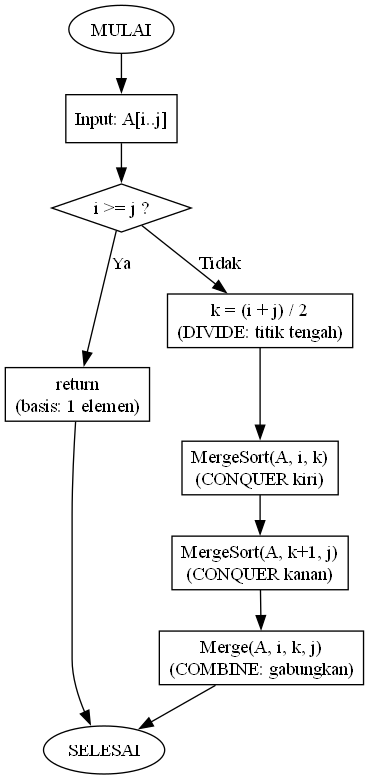
\includegraphics[width=0.45\textwidth]{figures/praktikum4/flowchart_mergesort.png}
    \caption{Flowchart Algoritma Merge Sort}
\end{figure}

\subsubsection*{Flowchart Quick Sort}
\begin{figure}[H]
    \centering
    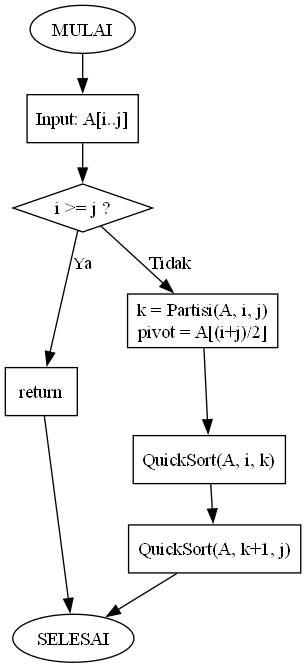
\includegraphics[width=0.45\textwidth]{figures/praktikum4/flowchart_quicksort.png}
    \caption{Flowchart Algoritma Quick Sort}
\end{figure}

\subsubsection*{Source Code Python: MinMaks D\&C}
\begin{lstlisting}[basicstyle=\ttfamily\scriptsize, frame=single, backgroundcolor=\color{white}, numbers=none, keywordstyle=\color{black}, commentstyle=\color{black}, stringstyle=\color{black}, breaklines=true]
def minmaks(arr, i, j):
    # basis: 1 elemen
    if i == j:
        return arr[i], arr[i]
        
    # basis: 2 elemen, bandingkan langsung
    if i == j - 1:
        if arr[i] < arr[j]:
            return arr[i], arr[j]
        else:
            return arr[j], arr[i]
            
    # rekursif: bagi tabel di titik tengah
    k = (i + j) // 2
    min1, maks1 = minmaks(arr, i, k)
    min2, maks2 = minmaks(arr, k + 1, j)
    
    # combine: ambil min dan maks dari kedua bagian
    return min(min1, min2), max(maks1, maks2)
\end{lstlisting}

\subsubsection*{Source Code Python: Merge Sort}
\begin{lstlisting}[basicstyle=\ttfamily\scriptsize, frame=single, backgroundcolor=\color{white}, numbers=none, keywordstyle=\color{black}, commentstyle=\color{black}, stringstyle=\color{black}, breaklines=true]
def merge(arr, kiri, tengah, kanan):
    # salin dua bagian ke array sementara
    kidal1 = arr[kiri:tengah + 1]
    kidal2 = arr[tengah + 1:kanan + 1]
    
    i = j = 0
    k = kiri
    
    # gabungkan dua bagian secara terurut
    while i < len(kidal1) and j < len(kidal2):
        if kidal1[i] <= kidal2[j]:
            arr[k] = kidal1[i]
            i += 1
        else:
            arr[k] = kidal2[j]
            j += 1
        k += 1
        
    # salin sisa elemen kiri jika ada
    while i < len(kidal1):
        arr[k] = kidal1[i]
        i += 1
        k += 1
        
    # salin sisa elemen kanan jika ada
    while j < len(kidal2):
        arr[k] = kidal2[j]
        j += 1
        k += 1

def merge_sort(arr, i, j):
    # basis: array 1 elemen sudah terurut
    if i >= j:
        return
        
    # divide: tentukan titik tengah
    k = (i + j) // 2
    
    # conquer: urutkan bagian kiri dan kanan secara rekursif
    merge_sort(arr, i, k)
    merge_sort(arr, k + 1, j)
    
    # combine: gabungkan hasil pengurutan
    merge(arr, i, k, j)
\end{lstlisting}

\subsubsection*{Source Code Python: Quick Sort}
\begin{lstlisting}[basicstyle=\ttfamily\scriptsize, frame=single, backgroundcolor=\color{white}, numbers=none, keywordstyle=\color{black}, commentstyle=\color{black}, stringstyle=\color{black}, breaklines=true]
def partisi(arr, i, j):
    # pilih elemen tengah sebagai pivot
    pivot = arr[(i + j) // 2]
    p, q = i, j
    
    while True:
        # scan dari kiri sampai menemukan elemen >= pivot
        while arr[p] < pivot:
            p += 1
        # scan dari kanan sampai menemukan elemen <= pivot
        while arr[q] > pivot:
            q -= 1
            
        # jika belum bertemu, tukar dan geser indeks
        if p < q:
            arr[p], arr[q] = arr[q], arr[p]
            p += 1
            q -= 1
        else:
            break
            
    return q

def quick_sort(arr, i, j):
    # basis: array 1 elemen atau kosong
    if i >= j:
        return
        
    # partisi dan dapatkan indeks pembagi
    k = partisi(arr, i, j)
    
    # rekursif urutkan bagian kiri dan kanan
    quick_sort(arr, i, k)
    quick_sort(arr, k + 1, j)

if __name__ == "__main__":
    data = [4, 12, 23, 9, 21, 1, 35, 2, 24]
    print("Data awal:", data)
    
    # MinMaks D&C
    mn, mx = minmaks(data, 0, len(data) - 1)
    print(f"\nMinMaks D&C -> Min: {mn}, Maks: {mx}")
    
    # Merge Sort
    arr_ms = data.copy()
    merge_sort(arr_ms, 0, len(arr_ms) - 1)
    print(f"Merge Sort -> {arr_ms}")
    
    # Quick Sort
    arr_qs = data.copy()
    quick_sort(arr_qs, 0, len(arr_qs) - 1)
    print(f"Quick Sort -> {arr_qs}")
\end{lstlisting}

\subsubsection*{Analisis Output}
Program dijalankan dengan data awal [4, 12, 23, 9, 21, 1, 35, 2, 24]:

\begin{table}[H]
    \centering
    \caption{Output Hasil Pengujian Algoritma Divide and Conquer}
    \begin{tabular}{p{3cm}p{5cm}p{6cm}}
    \toprule
    \textbf{Algoritma} & \textbf{Output} & \textbf{Keterangan} \\ \midrule
    MinMaks D\&C & Min: 1, Maks: 35 & Ditemukan dengan T(n) = O(n) perbandingan \\
    Merge Sort & [1, 2, 4, 9, 12, 21, 23, 24, 35] & Terurut stabil, O(n log n) \\
    Quick Sort & [1, 2, 4, 9, 12, 21, 23, 24, 35] & Terurut, rata-rata O(n log n) \\ \bottomrule
    \end{tabular}
\end{table}

\textbf{MinMaks D\&C:} Tabel dibagi dua pada k=4. Bagian kiri [4,12,23,9,21] menghasilkan min=4, maks=23. Bagian kanan [1,35,2,24] menghasilkan min=1, maks=35. Setelah combine: min=1, maks=35.

\textbf{Merge Sort:} Pembagian berlangsung rekursif hingga setiap bagian berukuran 1 elemen, lalu digabung secara terurut. Karena bersifat stabil, urutan relatif elemen bernilai sama terjaga.

\textbf{Quick Sort:} Pivot dipilih dari elemen tengah setiap iterasi. Proses partisi memindahkan elemen lebih kecil ke kiri dan lebih besar ke kanan pivot, kemudian kedua bagian diurutkan rekursif.

\subsection{Post Test: Merge Sort Standalone}

\subsubsection*{Source Code Python}
\begin{lstlisting}[basicstyle=\ttfamily\scriptsize, frame=single, backgroundcolor=\color{white}, numbers=none, keywordstyle=\color{black}, commentstyle=\color{black}, stringstyle=\color{black}, breaklines=true]
def merge(arr, kiri, tengah, kanan):
    # salin dua bagian ke array sementara
    bagian_kiri = arr[kiri:tengah + 1]
    bagian_kanan = arr[tengah + 1:kanan + 1]
    
    i = j = 0
    k = kiri
    
    # gabungkan dua bagian ke array utama secara terurut
    while i < len(bagian_kiri) and j < len(bagian_kanan):
        if bagian_kiri[i] <= bagian_kanan[j]:
            arr[k] = bagian_kiri[i]
            i += 1
        else:
            arr[k] = bagian_kanan[j]
            j += 1
        k += 1
        
    # salin sisa bagian kiri jika masih ada
    while i < len(bagian_kiri):
        arr[k] = bagian_kiri[i]
        i += 1
        k += 1
        
    # salin sisa bagian kanan jika masih ada
    while j < len(bagian_kanan):
        arr[k] = bagian_kanan[j]
        j += 1
        k += 1

def merge_sort(arr, i, j, depth=0):
    indent = "  " * depth
    # basis: array dengan 1 elemen sudah terurut
    if i >= j:
        return
        
    # divide: hitung titik tengah pembagi
    k = (i + j) // 2
    print(f"{indent}Divide [{i}..{j}] -> kiri [{i}..{k}], kanan [{k+1}..{j}]")
    
    # conquer: urutkan bagian kiri secara rekursif
    merge_sort(arr, i, k, depth + 1)
    
    # conquer: urutkan bagian kanan secara rekursif
    merge_sort(arr, k + 1, j, depth + 1)
    
    # combine: gabungkan hasil pengurutan kedua bagian
    merge(arr, i, k, j)
    print(f"{indent}Combine [{i}..{j}] -> {arr[i:j+1]}")

if __name__ == "__main__":
    data = [38, 27, 43, 3, 9, 82, 10]
    print("Data awal      :", data)
    print("\nProses Merge Sort (D&C):")
    print("-" * 45)
    
    merge_sort(data, 0, len(data) - 1)
    
    print("-" * 45)
    print("Data terurut   :", data)
\end{lstlisting}

\textbf{Jawaban 1: Trace proses Divide-Conquer-Combine}\\
Berikut trace verbose output program dengan data [38, 27, 43, 3, 9, 82, 10]:

\begin{table}[H]
    \centering
    \caption{Trace Eksekusi Merge Sort D\&C}
    \begin{tabular}{cll}
    \toprule
    \textbf{Langkah} & \textbf{Operasi} & \textbf{Hasil} \\ \midrule
    1 & Divide [0..6] -> kiri [0..3], kanan [4..6] & \\
    2 & Divide [0..3] -> kiri [0..1], kanan [2..3] & \\
    3 & Divide [0..1] -> kiri [0..0], kanan [1..1] & \\
    4 & Combine [0..1] & [27, 38] \\
    5 & Divide [2..3] -> kiri [2..2], kanan [3..3] & \\
    6 & Combine [2..3] & [3, 43] \\
    7 & Combine [0..3] & [3, 27, 38, 43] \\
    8 & Divide [4..5] -> kiri [4..4], kanan [5..5] & \\
    9 & Combine [4..5] & [9, 82] \\
    10 & Combine [4..6] & [9, 10, 82] \\
    11 & Combine [0..6] & [3, 9, 10, 27, 38, 43, 82] \\ \bottomrule
    \end{tabular}
\end{table}

\textbf{Jawaban 2: Output eksekusi}\\
Data awal: [38, 27, 43, 3, 9, 82, 10]. Setelah proses Merge Sort D\&C selesai, data terurut menjadi: [3, 9, 10, 27, 38, 43, 82]. Seluruh proses pembagian (Divide) dan penggabungan (Combine) ditampilkan verbose sehingga alur rekursi terlihat jelas dari kedalaman indentasi output.